%%%%%%%%%%%%%%%%%%%%%%%%%%%%%%%%%%%%%%%%%
% Programming/Coding Assignment
% LaTeX Template
%
% This template has been downloaded from:
% http://www.latextemplates.com
%
% Original author:
% Ted Pavlic (http://www.tedpavlic.com)
%
% Adapted by:
% Jacopo De Stefani (jacopo.de.stefani@gmail.com)
%
% Note:
% The \lipsum[#] commands throughout this template generate dummy text
% to fill the template out. These commands should all be removed when 
% writing assignment content.
%
% This template uses a Perl script as an example snippet of code, most other
% languages are also usable. Configure them in the "CODE INCLUSION 
% CONFIGURATION" section.
%
%%%%%%%%%%%%%%%%%%%%%%%%%%%%%%%%%%%%%%%%%

%----------------------------------------------------------------------------------------
%	PACKAGES AND OTHER DOCUMENT CONFIGURATIONS
%----------------------------------------------------------------------------------------

\documentclass{article}

\usepackage[utf8]{inputenc}
\usepackage{fancyhdr} % Required for custom headers
\usepackage{lastpage} % Required to determine the last page for the footer
\usepackage{extramarks} % Required for headers and footers
\usepackage[usenames,dvipsnames]{color} % Required for custom colors
\usepackage{graphicx} % Required to insert images
\usepackage{listings} % Required for insertion of code
\usepackage{courier} % Required for the courier font
\usepackage{lipsum} % Used for inserting dummy 'Lorem ipsum' text into the template
\usepackage{rotating}
\usepackage{natbib}
\usepackage{graphicx}
\usepackage{tikz}
\usepackage{pgfplots}
\usepackage{multicol}
\usepackage{caption}
\usepackage{amsmath}
\usepackage{amsfonts}
\usepackage{pdflscape}
\usepackage{hyperref}
\usepackage{pifont}

\usetikzlibrary{positioning,shadows,arrows,intersections,calc,automata}

% Margins
\topmargin=-0.45in
\evensidemargin=0in
\oddsidemargin=0in
\textwidth=6.5in
\textheight=9.0in
\headsep=0.25in

\linespread{1.1} % Line spacing

% Set up the header and footer
\pagestyle{fancy}
\lhead{} % Top left header
\chead{\hmwkClass\ (\hmwkClassInstructor\ ): \hmwkTitle} % Top center head
\rhead{}%\firstxmark} % Top right header
\lfoot{\hmwkAuthorName} % Bottom left footer
\cfoot{}%\lastxmark} % Bottom center footer
\rfoot{Page\ \thepage\ of\ \protect\pageref{LastPage}} % Bottom right footer
\renewcommand\headrulewidth{0.4pt} % Size of the header rule
\renewcommand\footrulewidth{0.4pt} % Size of the footer rule

\setlength\parindent{0pt} % Removes all indentation from paragraphs

%----------------------------------------------------------------------------------------
%	CODE INCLUSION CONFIGURATION
%----------------------------------------------------------------------------------------

\definecolor{MyDarkGreen}{rgb}{0.0,0.4,0.0} % This is the color used for comments
\lstloadlanguages{Python} % Load Perl syntax for listings, for a list of other languages supported see: ftp://ftp.tex.ac.uk/tex-archive/macros/latex/contrib/listings/listings.pdf
\lstset{language=Python, % Use Perl in this example
        frame=single, % Single frame around code
        basicstyle=\small\ttfamily, % Use small true type font
        keywordstyle=[1]\color{Blue}\bf, % Perl functions bold and blue
        keywordstyle=[2]\color{Purple}, % Perl function arguments purple
        keywordstyle=[3]\color{Blue}\underbar, % Custom functions underlined and blue
        identifierstyle=, % Nothing special about identifiers                                         
        commentstyle=\usefont{T1}{pcr}{m}{sl}\color{MyDarkGreen}\small, % Comments small dark green courier font
        stringstyle=\color{Purple}, % Strings are purple
        showstringspaces=false, % Don't put marks in string spaces
        tabsize=5, % 5 spaces per tab
        %
        % Put standard Perl functions not included in the default language here
        morekeywords={rand},
        %
        % Put Perl function parameters here
        morekeywords=[2]{on, off, interp},
        %
        % Put user defined functions here
        morekeywords=[3]{test},
       	%
        morecomment=[l][\color{Blue}]{...}, % Line continuation (...) like blue comment
        numbers=left, % Line numbers on left
        firstnumber=1, % Line numbers start with line 1
        numberstyle=\tiny\color{Blue}, % Line numbers are blue and small
        stepnumber=5, % Line numbers go in steps of 5
        breaklines=true
}

% Creates a new command to include a perl script, the first parameter is the filename of the script (without .pl), the second parameter is the caption
\newcommand{\pyscript}[2]{
\begin{itemize}
\item[]\lstinputlisting[caption=#2,label=#1]{#1.py}
\end{itemize}
}

%----------------------------------------------------------------------------------------
%	DOCUMENT STRUCTURE COMMANDS
%	Skip this unless you know what you're doing
%----------------------------------------------------------------------------------------

% Header and footer for when a page split occurs within a problem environment
\newcommand{\enterProblemHeader}[1]{
\nobreak\extramarks{#1}{#1 continued on next page\ldots}\nobreak
\nobreak\extramarks{#1 (continued)}{#1 continued on next page\ldots}\nobreak
}

% Header and footer for when a page split occurs between problem environments
\newcommand{\exitProblemHeader}[1]{
\nobreak\extramarks{#1 (continued)}{#1 continued on next page\ldots}\nobreak
\nobreak\extramarks{#1}{}\nobreak
}

\setcounter{secnumdepth}{0} % Removes default section numbers
\newcounter{homeworkProblemCounter} % Creates a counter to keep track of the number of problems

\newcommand{\homeworkProblemName}{}
\newenvironment{homeworkProblem}[1][Problem \arabic{homeworkProblemCounter}]{ % Makes a new environment called homeworkProblem which takes 1 argument (custom name) but the default is "Problem #"
\stepcounter{homeworkProblemCounter} % Increase counter for number of problems
\renewcommand{\homeworkProblemName}{#1} % Assign \homeworkProblemName the name of the problem
\section{\homeworkProblemName} % Make a section in the document with the custom problem count
\enterProblemHeader{\homeworkProblemName} % Header and footer within the environment
}{
\exitProblemHeader{\homeworkProblemName} % Header and footer after the environment
}

\newcommand{\problemAnswer}[1]{ % Defines the problem answer command with the content as the only argument
\noindent\framebox[\columnwidth][c]{\begin{minipage}{0.98\columnwidth}#1\end{minipage}} % Makes the box around the problem answer and puts the content inside
}

\newcommand{\homeworkSectionName}{}
\newenvironment{homeworkSection}[1]{ % New environment for sections within homework problems, takes 1 argument - the name of the section
\renewcommand{\homeworkSectionName}{#1} % Assign \homeworkSectionName to the name of the section from the environment argument
\subsection{\homeworkSectionName} % Make a subsection with the custom name of the subsection
\enterProblemHeader{\homeworkProblemName\ [\homeworkSectionName]} % Header and footer within the environment
}{
\enterProblemHeader{\homeworkProblemName} % Header and footer after the environment
}

%----------------------------------------------------------------------------------------
%	USER DEFINED TIKZ STYLES
%----------------------------------------------------------------------------------------

\tikzset{
    player1/.style={circle, draw=none, fill=green!70!black, circular drop shadow,
        text centered, anchor=north, text=white},
    player2/.style={circle, draw=none, fill=orange, circular drop shadow,
        text centered, anchor=north, text=white},
    chance/.style={circle, draw,text centered, anchor=north},
    subtreeB/.style={rectangle, draw, rounded corners=1mm, color=red, thick,
        text centered, anchor=north, text=red},
    subtreeC/.style={rectangle, draw, rounded corners=1mm, color=orange, thick,
        text centered, anchor=north, text=orange},
    ex2/.style={circle, draw,text centered, anchor=north},
    nashEq1P/.style={circle,draw=none, fill=green!70!black, text centered, anchor=north, text=white,inner sep=2pt},
    nashEq2P/.style={circle,draw=none, fill=orange, text centered, anchor=north, text=white,inner sep=2pt},
    nashEqPoints/.style={fill=white,draw=black,thick},
    level distance=0.5cm, growth parent anchor=south
}

\tikzstyle{tier}=[draw, fill=yellow!20, text width=6.0em, text centered,
  minimum height=1.5em,drop shadow]
\tikzstyle{component} = [tier, text width=8em, minimum width=10em,
  minimum height=3em, rounded corners, drop shadow,inner sep=2pt]
\tikzstyle{texto} = [above, text width=6em, text centered]
\tikzstyle{linepart} = [draw, thick, color=black!50, -latex', dashed]
\tikzstyle{line} = [draw, thick, color=black!50, -latex', ->]
\tikzstyle{ur}=[draw, text centered, minimum height=0.01em]
 
% Define distances for bordering
\newcommand{\blockdist}{1.3}
\newcommand{\edgedist}{1.5}

\newcommand{\component}[2]{node (p#1) [component]
  {{\scriptsize\textit{#2}}}}

% Draw background
\newcommand{\backgroundSquare}[5]{%
  \begin{pgfonlayer}{background}
    % Left-top corner of the background rectangle
    \path (#1.west |- #2.north)+(-0.5,0.5) node (a1) {};
    % Right-bottom corner of the background rectanle
    \path (#3.east |- #4.south)+(+0.5,-0.25) node (a2) {};
    % Draw the background
    \path[fill=blue!20,rounded corners, draw=black!50, dashed]
      (a1) rectangle (a2);
    \path (a1.east |- a1.south)+(0.8,-0.3) node (u1)[texto]
      {\scriptsize\textit{#5 Tier}};
  \end{pgfonlayer}}


\newcommand*\circled[2]{\tikz[baseline=(char.base)]{
            \node[#2,rectangle, rounded corners=0.7mm, text=white] (char) {#1};}}
\newcommand*\cellvcenter[1]{\raisebox{-\height}{#1}}


\newcommand{\cmark}{\ding{51}}%
\newcommand{\xmark}{\ding{55}}%

%----------------------------------------------------------------------------------------
%	NAME AND CLASS SECTION
%----------------------------------------------------------------------------------------

\newcommand{\hmwkTitle}{Implementation Exercise \#1 \\ The Traveling Salesman Problem with Time Windows} % Assignment title
\newcommand{\hmwkDueDate}{Wednesday,\ April\ 10,\ 2013} % Due date
\newcommand{\hmwkClass}{INFO-H-413 - Learning Dynamics} % Course/class
\newcommand{\hmwkClassTime}{} % Class/lecture time
\newcommand{\hmwkClassInstructor}{Prof. T. St\"{u}etzle} % Teacher/lecturer
\newcommand{\hmwkAuthorName}{Jacopo De Stefani} % Your name

%----------------------------------------------------------------------------------------
%	TITLE PAGE
%----------------------------------------------------------------------------------------

\title{
\vspace{2in}
\textmd{\textbf{\hmwkClass:\\ \hmwkTitle}}\\
%\normalsize\vspace{0.1in}\small{Due\ on\ \hmwkDueDate}\\
\vspace{0.1in}\large{\textit{\hmwkClassInstructor\ }}
\vspace{3in}
}

\author{\textbf{\hmwkAuthorName}}
\date{\today} % Insert date here if you want it to appear below your name

%----------------------------------------------------------------------------------------

\begin{document}

\maketitle

%----------------------------------------------------------------------------------------
%	TABLE OF CONTENTS
%----------------------------------------------------------------------------------------

%\setcounter{tocdepth}{1} % Uncomment this line if you don't want subsections listed in the ToC

\newpage
\tableofcontents
\newpage

\section{Implementation}

%----------------------------------------------------------------------------------------
%	PROBLEM 1
%----------------------------------------------------------------------------------------

% To have just one problem per page, simply put a \clearpage after each problem
\newpage
\begin{homeworkProblem}
\section{Iterative improvement algorithms}
\subsection{Problem statement}
To  understand  which  strategies  are  stable  against  invasion  implement  a   simulation  of  the  Moran  process  and  apply  it  to  modified  dictator  game. \\
Determine  for  each  strategy  xy  whether  it  is  stable  against  invasion.\\   
Send   the  simulation  code  and  the  results.           

\subsection{Simulation code}
The simulation code had been written using the Python programming language, in order to take advantage of the flexibility granted by dynamic typing system of the language.\\
This allowed me to focus on the details of the simulation, without having to deal with all the programming pitfalls of a strongly typed language.\\
The naming style adopted in the code is medial capitalization, starting from the second word, using full capital names to denote constant values, namely the simulation parameters.

\begin{center}
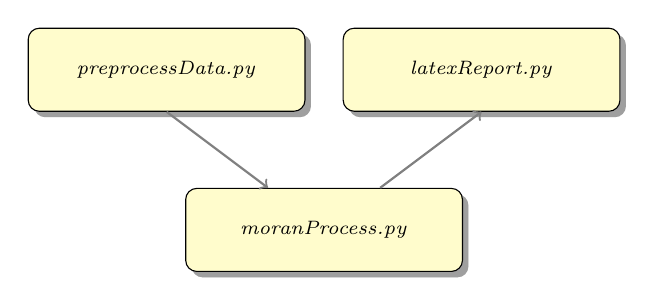
\begin{tikzpicture}[transform shape]
 
  % Draw diagram elements
  
  \path \component {1}{moranProcess.py};
  \path (p1.north)+(-2.0,+1.5) \component{2}{preprocessData.py};
  \path (p1.north)+(+2.0,+1.5) \component{3}{latexReport.py};
     
  % Draw arrows between elements
  \path [line] (p2.south) -> node [above] {} (p1);
  \path [line] (p1) -> node [above, midway] {} (p3.south);

  %\backgroundSquare{p1}{p1}{p3}{p3}{Presentation}

 \end{tikzpicture}
 \captionof{figure}{Simulation Code Structure}
\end{center}

The simulation code has been structured into three modules:
\begin{enumerate}
\item The input data preprocessing module - \emph{preprocessData.py}
\item The simulation module - \emph{moranProcess.py}
\item The result post-processing module - \emph{latexReport.py}
\end{enumerate}

\subsubsection{Relevant Parameters}
\begin{center}
\vskip7pt
\begin{tabular}{|l|c|c|}
\hline 
\textbf{Parameter} & \textbf{Value} & \textbf{Description} \\ \hline
$\alpha$ & 0.9 & Proportion of the split of the endowment\\ [10pt]
$P$ & $10^2$ & Endowment to split\\ [10pt]
$N$ & 50 & Population size \\ [10pt]
\emph{ITERATION} & $10^4$ & Number of iterations to be performed for each simulation\\ [10pt]
\emph{MAXSTEP} & $10\cdot N =$ 500 & Maximum number of step before considering the iteration non converging\\ [10pt]
$i$ & 1 & Initial number of A-type players\\ [10pt]
$w$ & 0.5 & Intensity of selection\\ [10pt]
\hline
\end{tabular}
\captionof{table}{Relevant parameters for the simulation}
\end{center}

\subsubsection{Input data preprocessing module}
The preprocessing module simply encodes the symmetric game payoff matrix determined in \ref{tab:spm} and automatically determines all the 36 pairwise comparisons among the pure strategies required as input data for the Moran Process to simulate.\\
The expected result, under the assumption of an infinite population, is determined for each of these generated simulations according to the values contained in the payoff matrix, following the results described in \cite{Taylor2004}, section 1.\\

%\pyscript{./Simulation/preprocessData}{}

\subsubsection{Simulation execution module}

\paragraph{Description}
This module contains all the necessary code to actually perform the simulation of the moran Process, namely the functions:
\begin{itemize}
\item \emph{simulationStepRelativeFitness()}
\item \emph{updateFitness()}
\end{itemize}

The simulation module obtains the preprocessed data from the corresponding module, then, for each of the 36 simulation:
\begin{enumerate}
\item Generates a population of $N$ individuals, $i$ of which of A-type.
\item Computes the initial fitness $f_A$ and $f_B$ of the population.
\item Performs \emph{ITERATION} runs of maximum $10*N$ simulation step each.
\item Calls the postprocessing module to produce a syntactically correct \LaTeX  file.
\end{enumerate}

\subparagraph{updateFitness()}
The expected payoff of A-type players, as in \cite{Taylor2004}, is determined as follows: 
\begin{equation}
p_A = a\cdot(i - 1) + b\cdot(N - i)
\end{equation}
while, for B-type players:
\begin{equation}
p_B = c\cdot i + d(N - i - 1)
\end{equation}
The fitness of each type of players is then determined according to \cite{Traulsen2010}:
\begin{equation}
\begin{array}{c}
f_A = 1-w+w\cdot p_A\\
f_B = 1-w+w\cdot p_B\\
\end{array}
\end{equation}
The intensity of selection $w \in [0,1]$ determines the relevance of the payoff in the computation of the fitness.\\
For the simulation it is chosen to be equal to $0.5$ in order neither to perform an individual duplication depending solely on the payoff ($w=1$) nor to have a completely random selection($w=0$).

\paragraph{simulationStepRelativeFitness()}
In each simulation step, an individual is selected at random to be eliminated and replaced by a copy of another existing individual in the population.\\
The duplication of an A-type individual occurs with a probability which is fitness dependant, as in \cite{Taylor2004}:
\begin{equation}
p_{D_A} = \frac{i \cdot f_A}{i \cdot f_A + (N-i)\cdot f_B}
\end{equation}
The number of A-type players is then adjusted according to the outcome of the probabilistic duplication.

%\pyscript{./Simulation/moranProcess}{}

\subsubsection{Output post-processing module}
At the end of each simulation, the functions of the \LaTeX post-processing module are called to produce the files, used to typeset the simulation results.\\
%\pyscript{./Simulation/latexReport}{}

\clearpage


\end{homeworkProblem}

\begin{homeworkProblem}
\section{Analysis of simulation results}
\label{sec:simres}
The following section presents the results of the simulation performed by executing the Python script.\\
One should remember, that the population is initialized with $1$ A-Type individual and $N-1$ B-Type individual.\\
At the end of every section, an overview of the results is shown stating:
\begin{itemize}
\item \textbf{Coherent}:
	\begin{itemize}
	\item \cmark - Whenever the expected result for an infinite population agrees with the results of the simulation.
	\item \xmark - If, due to some stochastic effect, the outcome of the simulation is different from what is expected.
	\end{itemize}
\item\textbf{Stable against invasion}:
	\begin{itemize}
	\item \cmark - Whenever the number of A-Type individuals converges to 0 at the end of the simulation.
	\item \xmark - If, either the invasion of a single A-Type individual can cause the extinction of B-Type players ($x_A=N$) or the stable state at the end of the simulation has a non null number of A-Type agents ($x_A=x^*$).
	\end{itemize}
\end{itemize}
It should be remarked that the outcome of the simulation is chosen to be the outcome having the greatest occurrence for each simulation.\\
Whenever there are other outcomes with a non negligible number of occurrences ($o_i>10^3$), the theoretical results and the experimental results are discordant. 
%\input{simulationResults}

\end{homeworkProblem}


%----------------------------------------------------------------------------------------
%	PROBLEM 2
%----------------------------------------------------------------------------------------
\begin{homeworkProblem}

\section{Variable Neighborhood Descent algorithms }
\subsection{Problem statement}
\subsubsection{Game description}
In  a  dictator  game  two  players  are  interacting.\\   
The  first  player  (also  called  the   proposer)  decides  on  how  some  endowment  is  split  between  the  players. \\
The   second  player  simply  receives  his  part  of  the  split. \\     
So  the  role  of  the  receiver  is   completely  passive,  no  decisions  have  to  be  taken  when  a  player  fulfills  that  role.
\\   We  assume  here  that  the  proposer  can  select  between  three  actions:    a  selfish,  a   fair   and   an   altruistic   split. \\
In   the   selfish   split,   she   keeps   the   majority   of   the   endowment  and  in  the  altruistic  action  she  hands  over  almost  all  the  endowment   to  the  receiver. \\ 
In  the  fair  case,  she  splits  the  endowment  in  an  equal  manner. \\        
As  opposed  to  the  normal  Dictator  Game,  we  will  now  assume  here  that  in  this   game,  before  the  dictator  proposes  a  split,  the  player  needs  to  decide  whether  he   or  she  wants  to  play  the  game.  So  now  the  player  has  two  actions  “play”  or    “not   play”. \\
If  the  receiver  decides  to  play,  the  proposer  simply  decides  the  split.  If  the   receiver  decides  not  to  play  both  get  zero  payoff.     

\subsubsection{Part I}
\begin{enumerate}
\item Draw  the  Extensive  Form  Game  that  corresponds  and  report  the  Subgame  Perfect  equilibrium. 
\item Create   the   Strategic   Form   of   this   game   and   determine   the   Nash  Equilibrium  of  this  game. 
\end{enumerate}


\subsubsection{Part II}
The  game  is  clearly  not  symmetric. Yet  we  can  make  it  so. \\    We  need  to  assume   that  a  strategy  takes  the  role  of  the  player  into  account. \\
When  two  players  meet   their  role  is  randomly  assigned.  A  pure  strategy  of  for  each  of  these  players  can   be  written  as  ‘xy’  which  means  ‘if  I  am  the  proposer  I  play  x  if  I  am  the  receiver  I   play  y’,  where  the  ‘x’  is  either  ‘selfish  split’  (S),  ‘altruistic  split’  (A)    or  ‘Fair  split’   (F)  and  the  ‘y’  is  either  ‘Play  (P)  or    ‘Don’t  play’  (N).\\    
The  payoff  they  receive  is   the  mean  of  the  payoffs  for  both  choices.     
\begin{enumerate}
\item How  many  pure  strategies  are  there  for  each  player? 
\item Write   down   the   normal   form   and   determine   the   Nash   equilibria   of   this  game. 
\end{enumerate}

\subsection{Proposed solution}
\subsubsection{Question 1}
\paragraph{Modeling assumptions}
\label{par:modeling}
The original Dictator game is formally a two-players degenerate game, in the sense that the outcome of the game does not depend on the choices made by all the players in the game, with the second player having a completely passive role.\\
The proposed modification makes the problem a proper sequential game, thus allowing one to represent it using the extensive form model.\\
The consider game has two players, each of them having a set of possible actions:
\begin{itemize}
\item Proposer ($P_r$) : \{\emph{Selfish split}(S), \emph{Fair split}(F), \emph{Altruistic split}(A)\}
\item Receiver ($R_e$) : \{\emph{Don't play}(N), \emph{Play}(P)\}
\end{itemize}
To model the split proposed by $P_r$, two parameters are used:
\begin{enumerate}
\item $P \in \mathbb{N}^+$ - The endowment to split among the players
\item $\alpha \in (0.5,1)$ - The ratio of the split taken by the proposer.
\end{enumerate} 
As one may notice, the part of the endowment taken by the proposer and the receiver can be expressed, respectively as $\alpha P$ and $(1-\alpha) P$ such that $\alpha P+(1-\alpha) P = P$.\\
Moreover, by restricting the admissible set of values for $\alpha$, it is guaranteed that one player will get a larger part of the good with respect to the other one (the proposer in the \emph{Selfish split},the receiver in the \emph{Altruistic split}). \\
The \emph{Altruistic split} correspond to a \emph{Selfish split} where the payoff of the players are switched. \\ 
On the other hand, the \emph{Fair split} corresponds to the case $\alpha=0.5$, yielding to an equal split of the endowment. \\

\begin{center}
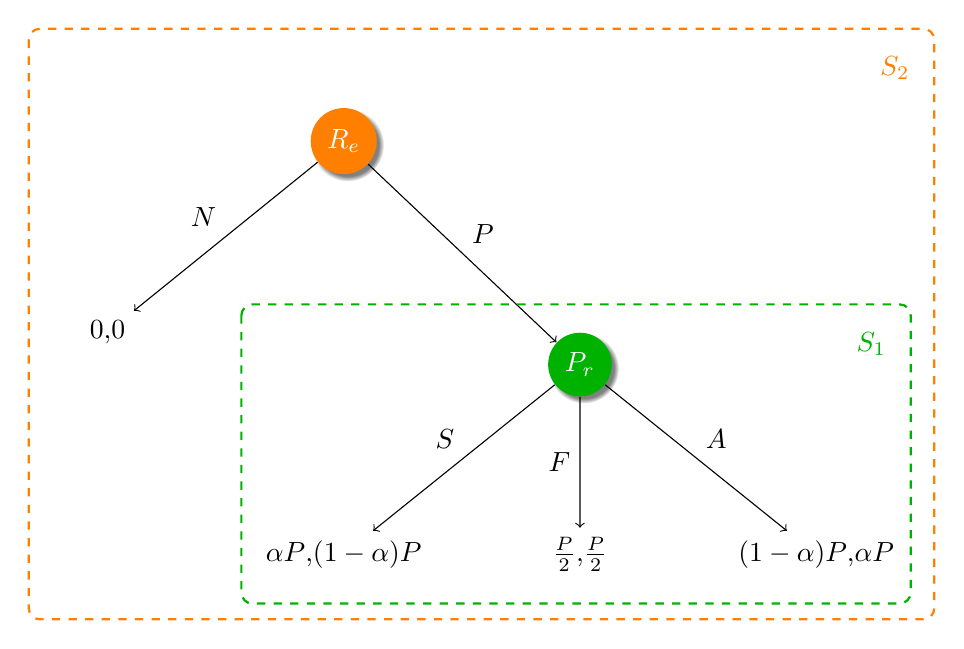
\begin{tikzpicture}
\tikzstyle{level 1}=[level distance=2cm, sibling distance=6cm]
\tikzstyle{level 2}=[level distance=2cm, sibling distance=3cm]
\tikzstyle{level 3}=[level distance=2cm, sibling distance=3cm]
\tikzstyle{level 4}=[level distance=2cm, sibling distance=3cm]

\node (root) [player2] {$R_e$} [->]
    child{
      		  node (leaf3) {0,0}
      		  edge from parent
      		   	node[above left] {$N$}
	   }
   child{
   		  node (1P) [player1] {$P_r$}
   		  child{
   		  		node (leaf3) {$\alpha P$,$(1-\alpha) P$}
      		  		edge from parent
      		   			node[above left] {$S$}
   		  }
   		  child{
   		  		node (leaf3) {$\frac{P}{2}$,$\frac{P}{2}$}
      		  		edge from parent
      		   			node[left] {$F$}
   		  }
   		  child{
   		  		node (leaf3) {$(1-\alpha) P$,$\alpha P$}
      		  		edge from parent
      		   			node[above right] {$A$}
   		  }
   		  edge from parent
      		   	node[above right] {$P$}
        };
        

\path [rounded corners, draw=orange, thick,dashed]
            (-4,1) rectangle (7.5,-6.5);
\node at (7,0.5) [text=orange, thick] {$S_2$};

\path [rounded corners, draw=green!70!black, thick,dashed]
            (-1.3,-2.5) rectangle (7.2,-6.3);
\node at (6.7,-3) [text=green!70!black, thick] {$S_1$};
\end{tikzpicture}
\captionof{figure}{Extensive form representation for modified dictator game}
\label{fig:spe}
\end{center}

The depicted extensive game consists of :
\begin{itemize} 
\item a set of players \{$P_r$, $R_e$\}
\item a set of terminal histories with the property that none of these histories
is a proper sub-history of another - \{\emph{Don't play}(N), (\emph{Play},\emph{Selfish split})(P,S), (\emph{Play},\emph{Fair split})(P,F), (\emph{Play},\emph{Altruistic split})(P,A)\}
\item a player function that assigns a player to every proper sub-history that can be derived from the terminal histories - $P(\emptyset) =$ \{$R_e$\}, $P($\emph{Play}$) =$ \{$P_r$, $R_e$\}
\item for each player, preferences over the set of terminal histories:
	 \begin{itemize}
	 \item $P_r$ (P,S) $>$ (P,F) $>$ (P,A) $>$ N 
	 \item $R_e$ (P,A) $>$ (P,F) $>$ (P,S) $>$ N
	 \end{itemize}
\end{itemize}

\paragraph{Equilibria analysis}
Prior to the computation of the subgame perfect equilibria, one has to determine the number of subgames which compose the analyzed problem.\\
In the considered game there are two subgames:
\begin{itemize}
\item $S_1$
\item $S_2$
\end{itemize}
The backward induction algorithm used to compute the subgame perfect equilibrium of $S_2$  requires the computation of the subgame perfect equilibrium for the nested subgame $S_1$.\\
To summarize, the subgame perfect equilibria corresponding to the game is indeed (\emph{Play}, \emph{Selfish split}), according to the aforementioned preferences, since :
\begin{itemize}
\item (BI - Step one) \emph{Selfish split} action is the subgame perfect equilibrium of subgame $S_1$ since it gives to the $P_r$ player the larger part of the endowment, considered all the other actions. 
\item (BI - Step two) The \emph{Play} action is the subgame perfect equilibrium of subgame $S_2$ since player $R_e$ is asked to choose between receiving a small part of the endowment or a null part of it, thus selecting the non null split (as long as $\alpha \ne 1$, case excluded according to modeling assumptions).
\end{itemize}


\subsubsection{Question 2}
\paragraph{Normal form representation}
The modified dictator game can be represented as a normal form, assuming that the two players are playing simultaneously.\\
As described in \ref{par:modeling} there are two players ($P_r$ and $R_e$) having respectively three (S,F,A) and two (N,P) actions, yielding to the following strategic form:
\begin{center}
\begin{tabular}{|l|c|c|}
\hline
& \textbf{N} & \textbf{P} \\ \hline
\textbf{S} & 0,0 & $\alpha P$,$(1-\alpha) P$ \\ \hline
\textbf{F} & 0,0 & $\frac{P}{2}$,$\frac{P}{2}$ \\ \hline
\textbf{A} & 0,0 & $(1-\alpha) P$,$\alpha P$ \\ \hline
  \end{tabular}
\captionof{table}{Normal (Strategic) form for modified dictator game}
\label{tab:normform}
\end{center}
Whenever $R_e$ decides not to play, both the player will get a null payoff, otherwise they can be deduced in a straightforward fashion from the extensive form representation.

\paragraph{Nash equilibrium determination}

The Nash equilibrium for the game can be computed by determining the best response sets for each player and then selecting action profiles $a^*$ in which every action is a best response to the other player's actions.\\
\begin{center}
\begin{tabular}{|l|c|c|}
\hline
& \textbf{N} & \textbf{P} \\ \hline
\textbf{S} & \circled{0}{nashEq1P},0 & \circled{$\alpha P$}{nashEq1P},\circled{$(1-\alpha) P$}{nashEq2P} \\ \hline
\textbf{F} & \circled{0}{nashEq1P},0 & $\frac{P}{2}$,\circled{$\frac{P}{2}$}{nashEq2P} \\ \hline
\textbf{A} & \circled{0}{nashEq1P},0 & $(1-\alpha) P$,\circled{$\alpha P$}{nashEq2P} \\ \hline
  \end{tabular}
\captionof{table}{Best response analysis on the normal form of the modified dictator game}
\label{tab:bra}
\end{center}
\subparagraph{Player $\mathbf{P_r}$}
\begin{tabular}{c c}
$B_{P_{r}}(N)$ = \{S, F, A\} & $B_{P_{r}}(P)$ = \{S\}\\
\end{tabular}

\subparagraph{Player $\mathbf{R_e}$}
\begin{tabular}{c c c}
$B_{R_{e}}(S)$ = \{P\} & $B_{R_{e}}(F)$ = \{P\} & $B_{R_{e}}(A)$ = \{P\}\\
\end{tabular}\\

Since $B_{R_{e}}(S)$ = \{P\} and $B_{P_{r}}(P)$ = \{S\} the only Nash equilibrium of the game is \emph{Selfish split},\emph{Play}.\\
This result is justified by the fact that every subgame perfect equilibrium is a Nash Equilibrium as well.

\subsection{Proposed solution  - Part II}
\subsubsection{Question 1}
A game is defined as symmetrical if, denoted with $A$ and $B$ respectively the payoff matrices of player $P_r$ and $R_e$, one has $A=B^T$. \\
As suggested in the problem formulation, the game can be transformed into an equivalent symmetric game by assuming that the player's role is randomly assigned (i.e. every player act 50\% of the time as a row player and 50\% of the time as a column player.\\
Hence, both players must have the same number of pure strategies in the form $xy$, where $x$ is a pure strategy for player $P_r$ and  $x$ is a pure strategy for player $R_e$.\\
Indicating with $A_i$ the action set for player $i$, one has:
\begin{itemize}
\item $A_{P_r}$ : \{\emph{Selfish split}(S),\emph{Fair split}(F),\emph{Altruistic split}(A)\}
\item $A_{R_e}$ :  \{\emph{Don't play}(N),\emph{Play}(P)\}
\end{itemize}
Given that $|A_{P_r}| = 3$ and $|A_{R_e}| = 2$ the pure strategy set for the symmetrical game corresponds to the Cartesian product of the players' pure strategy sets:
\begin{equation} 
A_s = A_{P_r}\times A_{R_e} =  \{(S,N), (S,P), (F,N), (F,P), (A,N), (A,P)\}\\
\end{equation}
hence the number of pure strategies is:
\begin{equation} 
|A_s| =|A_{P_r}|\cdot|A_{R_e}|=6
\end{equation}

\subsubsection{Question 2}
The normal form of symmetrical game is a 6x6 table, where the payoffs are determined as the average payoff that the players will receive acting one time as column player and the other time as row player as follows:
\begin{equation} 
U_s(x_1y_1,x_2y_2) = \frac{U_{P_r}(x_1,y_1)+U_{R_e}(x_2,y_2)}{2}
\end{equation}
$U_{P_r}(x,y)$ and $U_{R_e}(x,y)$ are the payoff for players $P_r$ and $R_e$ respectively as in table \ref{tab:normform}.\\ 
As described in the problem statement, the  payoff  they receive  is   the  mean  of  the  payoffs  for  both  choices.\\    
The details of computations are reported in the following table.
\newpage
\begin{landscape}
\begin{center}
\label{tab:spm}
\begin{tabular}{|l|c|c|c|c|c|c|}
\hline
& \textbf{SN} & \textbf{SP} & \textbf{FN} & \textbf{FP} & \textbf{AN} & \textbf{AP} \\ \hline
%Eerste rij
\cellvcenter{\textbf{SN}} &\cellvcenter{0,0} & \cellvcenter{$(1-\alpha)\frac{P}{2}$,$(1-\alpha)\frac{P}{2}$} & \cellvcenter{0,0} & \cellvcenter{$\frac{P}{4}$,$\frac{P}{4}$} & \cellvcenter{0,0} & \cellvcenter{$\frac{\alpha P}{2}$,\circled{$\frac{\alpha P}{2}$}{nashEq2P}} \\ [10pt] \hline 
%Tweede rij
\cellvcenter{\textbf{SP}} & \cellvcenter{\circled{$\frac{\alpha P}{2}$}{nashEq1P},$\frac{\alpha P}{2}$} & \cellvcenter{\circled{$\frac{P}{2}$}{nashEq1P},$\frac{P}{2}$} & \cellvcenter{\circled{$\frac{\alpha P}{2}$}{nashEq1P},$\frac{\alpha P}{2}$} & \cellvcenter{\circled{$\frac{(2\alpha+1)P}{4}$}{nashEq1P},$\frac{(2\alpha+1)P}{4}$} & \cellvcenter{\circled{$\frac{\alpha P}{2}$}{nashEq1P},$\frac{\alpha P}{2}$} & \cellvcenter{\circled{$\alpha P$}{nashEq1P},\circled{$\alpha P$}{nashEq2P}} \\ [10pt] \hline
%Derde rij
\cellvcenter{\textbf{FN}} & \cellvcenter{0,0} & \cellvcenter{$(1-\alpha)\frac{P}{2}$,$(1-\alpha)\frac{P}{2}$} & \cellvcenter{0,0} & \cellvcenter{$\frac{P}{4}$,$\frac{P}{4}$} & \cellvcenter{0,0} & \cellvcenter{$\frac{\alpha P}{2}$,\circled{$\frac{\alpha P}{2}$}{nashEq2P}} \\ [10pt]\hline
%Vierde rij
\cellvcenter{\textbf{FP}} &  \cellvcenter{$\frac{P}{4}$,$\frac{P}{4}$} & \cellvcenter{$(\frac{3}{2}-\alpha)\frac{P}{2}$,$(\frac{3}{2}-\alpha)\frac{P}{2}$} &\cellvcenter{$\frac{P}{4}$,$\frac{P}{4}$} & \cellvcenter{$\frac{P}{2}$,$\frac{P}{2}$} & \cellvcenter{$\frac{P}{4}$,$\frac{P}{4}$} & \cellvcenter{$\frac{(2\alpha+1)P}{4}$,\circled{$\frac{(2\alpha+1)P}{4}$}{nashEq2P}}\\ [10pt] \hline
%Vijfde rij
\cellvcenter{\textbf{AN}} & \cellvcenter{0,0} & \cellvcenter{$(1-\alpha)\frac{P}{2}$,$(1-\alpha)\frac{P}{2}$} & \cellvcenter{0,0} & \cellvcenter{$\frac{P}{4}$,$\frac{P}{4}$} & \cellvcenter{0,0} & \cellvcenter{$\frac{\alpha P}{2}$,\circled{$\frac{\alpha P}{2}$}{nashEq2P}} \\ [10pt] \hline
%Zesde rij
\cellvcenter{\textbf{AP}} &  \cellvcenter{$(1-\alpha)\frac{P}{2}$,$(1-\alpha)\frac{P}{2}$}  & \cellvcenter{$(1-\alpha)P$,$(1-\alpha)P$} & \cellvcenter{$(1-\alpha)\frac{P}{2}$,$(1-\alpha)\frac{P}{2}$ } & \cellvcenter{ $(\frac{3}{2}-\alpha)\frac{P}{2}$,$(\frac{3}{2}-\alpha)\frac{P}{2}$}  &  \cellvcenter{$(1-\alpha)\frac{P}{2}$,$(1-\alpha)\frac{P}{2}$} & \cellvcenter{$\frac{P}{2}$,\circled{$\frac{P}{2}$}{nashEq2P}} \\ [10pt] \hline
  \end{tabular}
\captionof{table}{Normal (Strategic) form for modified dictator game after symmetric transformation}
\end{center}
\vskip10pt
The Nash Equilibria of the game are determined by means of the best response analysis in the same manner as already done in table \ref{tab:bra}.\\
The total ordering of the payoff values, under the assumption that $\alpha \in (0.5,1)$, are included in table \ref{tab:bra1P} and table \ref{tab:bra2P}, along with the best response for every player, to each action.\\
\begin{itemize}
\item \textbf{1P} : SP - \textbf{2P} : AP
\end{itemize}
One should recall that, for player $i$, the strategy \emph{xy} signifies that, if player $i$ is the proposer, then it should play action \emph{x}.\\
On the other hand, if it is the receiver, it should play the strategy \emph{y}.\\
To be coherent with the previous analysis one can assume 1P$\equiv P_r$ and 2P$ \equiv R_e$ which yields to:
\begin{itemize}
\item $\mathbf{P_r}$ : S (\emph{Selfish split}) - $\mathbf{R_e}$ : P(Play)
\end{itemize}
The unique Nash equilibrium for the symmetric game is equal to the one determined in figure \ref{fig:spe} and table \ref{tab:bra}.
\end{landscape}
\clearpage

\textbf{Player 1}
\begin{center}
\vskip7pt
\begin{tabular}{|l|c|c|}
\hline 
\textbf{Action} & \textbf{Payoff Order} & \textbf{Best Response} \\ \hline
\textbf{SN}$\mathbf{(\alpha > \frac{2}{3})}$ & $\frac{\alpha P}{2}>\frac{\alpha P}{4}>(1-\alpha)\frac{P}{2}$ & \textbf{SP}\\ [10pt]
\textbf{SN}$\mathbf{(\alpha < \frac{2}{3})}$ & $\frac{\alpha P}{2}>(1-\alpha)\frac{P}{2}>\frac{\alpha P}{4}$ & \textbf{SP}\\ [10pt]
\textbf{SP} & $\frac{P}{2}>(\frac{3}{2}-\alpha)\frac{P}{2}>(1-\alpha)P>(1-\alpha)\frac{P}{2}$ & \textbf{SP}\\ [10pt]
\textbf{FN}$\mathbf{(\alpha > \frac{2}{3})}$ & $\frac{\alpha P}{2}>\frac{\alpha P}{4}>(1-\alpha)\frac{P}{2}$ & \textbf{SP}\\ [10pt] 
\textbf{FN}$\mathbf{(\alpha < \frac{2}{3})}$ & $\frac{\alpha P}{2}>(1-\alpha)\frac{P}{2}>\frac{\alpha P}{4}$ & \textbf{SP}\\ [10pt]
\textbf{FP} & $(2\alpha+1)\frac{P}{4}>\frac{P}{2}>\frac{P}{4}>(\frac{3}{2}-\alpha)\frac{P}{2}$ & \textbf{SP}\\ [10pt]
\textbf{AN}$\mathbf{(\alpha > \frac{2}{3})}$ & $\frac{\alpha P}{2}>\frac{\alpha P}{4}>(1-\alpha)\frac{P}{2}$ & \textbf{SP}\\ [10pt]
\textbf{AN}$\mathbf{(\alpha < \frac{2}{3})}$ & $\frac{\alpha P}{2}>(1-\alpha)\frac{P}{2}>\frac{\alpha P}{4}$ & \textbf{SP}\\ [10pt]
\textbf{AP} & $\alpha P>(2\alpha+1)\frac{P}{4}>\frac{P}{2}>\frac{\alpha P}{2}$ & \textbf{SP}\\ [10pt]
\hline
\end{tabular}
\captionof{table}{Best response analysis for player 1}
\label{tab:bra1P}
\end{center}

\textbf{Player 2}
\begin{center}
\vskip7pt
\begin{tabular}{|l|c|c|}
\hline 
\textbf{Action} & \textbf{Payoff Order} & \textbf{Best Response} \\ \hline
\textbf{SN} & $\frac{\alpha P}{2}>\frac{P}{4}>(1-\alpha)\frac{P}{2}$ & \textbf{AP}\\ [10pt]
\textbf{SP} & $\alpha P>(2\alpha+1)\frac{P}{4}>\frac{P}{2}>\frac{\alpha P}{2}$ & \textbf{AP}\\ [10pt]
\textbf{FN} & $\frac{\alpha P}{2}>\frac{P}{4}>(1-\alpha)\frac{P}{2}$ & \textbf{AP}\\ [10pt]
\textbf{FP} & $(2\alpha+1)\frac{P}{4}>\frac{P}{2}>\frac{P}{4}>(\frac{3}{2}-\alpha)\frac{P}{2}$ & \textbf{AP}\\ [10pt]
\textbf{AN} & $\frac{\alpha P}{2}>\frac{P}{4}>(1-\alpha)\frac{P}{2}$ & \textbf{AP}\\ [10pt]
\textbf{AP} & $\frac{P}{2}>(\frac{3}{2}-\alpha)\frac{P}{2}>(1-\alpha)P>(1-\alpha)\frac{P}{2}$ & \textbf{AP}\\ [10pt]
\hline
\end{tabular}
\captionof{table}{Best response analysis for player 2}
\label{tab:bra2P}
\end{center}

\end{homeworkProblem}		

\section{Conclusion}

\bibliographystyle{plain}
\bibliography{Assignment2}

\end{document}